\chapter{Eigenvalue Problem} \label{chap:polynomial-eigenvalue-problem}
In previous chapter, Chap.~\ref{chap:fluid-equations}, we derived the governing equations for the plasma flow in the magnetic nozzle. We also discussed the velocity profiles of the steady flows in the nozzle. In this chapter, we proceed to linearize these governing equations and reframe the problem as an eigenvalue problem. More specifically, a polynomial eigenvalue problem. Finally, we explore analytically a special case where the plasma flows with constant velocity under two boundary conditions, Dirichlet boundary and fixed-open boundary.

\section{Linearized Governing Equations}
As illustrated in Sec.\ref{sec:instability-of-plasma-flow}, it is essential to linearize the governing equations in order to investigate the linear instability of plasma. Now we are going to derive the linearized governing equations with the equilibrium conditions given in above.

Let $n = n_0(z) + \tilde{n}(z,t)$ and $v = v_0(z) + \tilde{v}(z,t)$, where $\tilde{n}$ and $\tilde{v}$ are small perturbed quantities.

We first linearize Eq.~(\ref{eq:conservation-of-density}) by setting $n=n_0+\tilde{n}$ and $v=v_0+\tilde{v}$,
\[    \pdv{(n_0+\tilde{n})}{t}
	+ (n_0+\tilde{n})\pdv{(v_0+\tilde{v})}{z}
	+ (v_0+\tilde{v})\pdv{(n_0+\tilde{n})}{z}
	- (n_0+\tilde{n})(v_0+\tilde{v})\frac{\partial_z B}{B} = 0
\]
By ignoring the nonlinear terms, we obtain
\[ \frac{1}{n_0}\pdv{\tilde{n}}{t}
	+ \pdv{v_0}{z} + \frac{\tilde{n}}{n_0}\pdv{v_0}{z} + \pdv{\tilde{v}}{z}
	+ \frac{v_0}{n_0}\pdv{n_0}{z} + \frac{\tilde{v}}{n_0}\pdv{n_0}{z} + \frac{v_0}{n_0}\pdv{\tilde{n}}{z}
	- v_0\frac{\partial_z B}{B} - \tilde{v}\frac{\partial_z B}{B} - \tilde{n}\frac{v_0}{n_0}\frac{\partial_z B}{B} = 0
\]

Using the equilibrium condition Eq.~(\ref{eq:equilibrium-conservation-of-density}), $\partial_zv_0+v_0\partial_zn_0/n_0$ cancels $-v_0\partial_zB/B$,
\[ \frac{1}{n_0}\pdv{\tilde{n}}{t}
	+ \frac{\tilde{n}}{n_0}\pdv{v_0}{z} + \pdv{\tilde{v}}{z}
	+ \frac{\tilde{v}}{n_0}\pdv{n_0}{z} + \frac{v_0}{n_0}\pdv{\tilde{n}}{z}
	- \tilde{v}\frac{\partial_z B}{B} - \tilde{n}\frac{v_0}{n_0}\frac{\partial_z B}{B} = 0
\]

Moreover, the last term can be written as
\[ \tilde{n}\frac{v_0}{n_0}\frac{\partial_z B}{B} = \frac{\tilde{n}}{n_0}\left( \frac{\partial_z n_0}{n_0}v_0 + \pdv{v_0}{z} \right) \]
Now, we get the linearized conservation of mass,
\begin{equation} \label{eq:linearized-conservation-of-density}
	\frac{1}{n_0}\pdv{\tilde{n}}{t}
	+ \pdv{\tilde{v}}{z} + v_0\tilde{Y} + \tilde{v}\frac{\partial_z n_0}{n_0} - \tilde{v}\frac{\partial_z B}{B} = 0
\end{equation}
where
\[ \tilde{Y} \equiv \frac{1}{n_0}\pdv{\tilde{n}}{z} - \frac{\partial_z n_0}{n_0^2}\tilde{n} = \pdv{z}(\frac{\tilde{n}}{n_0}) \]

To linearize the conservation of momentum, we follow the same logic by substituting $n=n_0+\tilde{n}$, and $v=v_0+\tilde{v}$ in Eq.~(\ref{eq:conservation-of-momentum}),
\[ (n_0+\tilde{n})\pdv{(v_0+\tilde{v})}{t} + (n_0+\tilde{n})(v_0+\tilde{v})\pdv{(v_0+\tilde{v})}{z} = -\pdv{(n_0+\tilde{n})}{z} \]

Again, ignore second order perturbations and rearrange terms, we have
\[ \pdv{\tilde{v}}{t} + v_0\pdv{\tilde{v}}{z} + \tilde{v}\pdv{v_0}{z}
	= -\frac{1}{n_0}\pdv{n_0}{z} -\frac{1}{n_0}\pdv{\tilde{n}}{z} -v_0\pdv{v_0}{z} - \frac{\tilde{n}}{n_0}v_0\pdv{v_0}{z} \]
Using the equilibrium condition Eq.~(\ref{eq:equilibrium-conservation-of-momentum}) on the RHS, we get the linearized conservation of momentum,
\begin{equation} \label{eq:linearized-conservation-of-momentum}
	\pdv{\tilde{v}}{t} + \pdv{(v_0\tilde{v})}{z} = -\tilde{Y}
\end{equation}

\section{Polynomial Eigenvalue Problem}
We can further simplify the problem by combining Eq.~(\ref{eq:linearized-conservation-of-density}) and Eq.~(\ref{eq:linearized-conservation-of-momentum}) into a single equation. We can substitute Eq.~(\ref{eq:linearized-conservation-of-momentum}) into Eq.~(\ref{eq:linearized-conservation-of-density}) to eliminate $\tilde{Y}$,

\begin{equation} \label{eq:single-governing-equation}
	\pdv{t}\frac{\tilde{n}}{n_0}
	+ \pdv{\tilde{v}}{z} - v_0\left(\pdv{t}\tilde{v}
	+ \pdv{(v_0\tilde{v})}{z}\right)
	+ \tilde{v}\frac{\partial_z n_0}{n_0}
	- \tilde{v}\frac{\partial_z B}{B}
	= 0
\end{equation}

In order to investigate the linear instability of the flow, we need to formulate it as an eigenvalue problem. To do that, we assume the perturbed density and velocity are oscillatory, i.e. $\tilde{n}, \tilde{v} \sim \exp(-i\omega t)$, where $\omega$ is the oscillation frequency of the perturbed quantities. This frequency can be a complex number.

As illustrated in Sec.\ref{sec:instability-of-plasma-flow}, the flow can be stable or unstable depending on the imaginary part of the frequency. If $\Im(\omega) > 0$, then the perturbed quantities $\tilde{n} \sim \exp(\Im(\omega) t)$, which means it grows exponentially with time, hence unstable. If $\Im(\omega) \leq 0$, then the amplitude of the perturbed quantities are either unchanged or exponentially decreasing, hence the flow is stable.

By assuming oscillatory perturbed quantities, Eq.~(\ref{eq:single-governing-equation}) becomes,
\begin{equation}
	-i\omega\frac{\tilde{n}}{n_0}
	+ \pdv{\tilde{v}}{z} - v_0\left(-i\omega\tilde{v}
	+ \pdv{(v_0\tilde{v})}{z}\right)
	+ \tilde{v}\frac{\partial_z n_0}{n_0}
	- \tilde{v}\frac{\partial_z B}{B}
	= 0
\end{equation}

Using the equilibrium condition Eq.~(\ref{eq:equilibrium-conservation-of-density}), we can eliminate the term $\partial_z B/B$,
\[
	-i\omega\frac{\tilde{n}}{n_0}
	+ \pdv{\tilde{v}}{z}
	+ v_0\left(i\omega \tilde{v} - v_0\pdv{\tilde{v}}{z} - \tilde{v}\pdv{v_0}{z} \right)
	- \tilde{v}\frac{\partial_z v_0}{v_0}
	= 0
\]

Rearrange terms, we have
\begin{equation}
	-i\omega\frac{\tilde{n}}{n_0}
	+ i\omega v_0\tilde{v}
	+ (1-v_0^2)\pdv{\tilde{v}}{z}
	- \left(v_0+\frac{1}{v_0}\right)\pdv{v_0}{z}\tilde{v} = 0
	\label{eq:intermediate-step-time-derivative-of-Y}
\end{equation}

Now we take $\pdv*{t}$ on Eq.~(\ref{eq:linearized-conservation-of-momentum}). Recall the fact that $\tilde{Y} = \partial_z(\tilde{n}/n_0)$, we have
\[
	\omega^2\tilde{v} + i\omega\left(v_0\pdv{\tilde{v}}{z} + \tilde{v}\pdv{v_0}{z}\right)
	= \pdv{t}\pdv{z}(\frac{\tilde{n}}{n_0})
\]
Switch the order of $\partial_t$ and $\partial_z$, and recall $-i\omega \tilde{n}/n_0$ can be obtained from Eq.~(\ref{eq:intermediate-step-time-derivative-of-Y}), we get
\[
	\omega^2\tilde{v} + i\omega\left(v_0\pdv{\tilde{v}}{z} + \tilde{v}\pdv{v_0}{z}\right)
	= \pdv{z}(-i\omega v_0\tilde{v}
	- (1-v_0^2)\pdv{\tilde{v}}{z}
	+ \left(v_0+\frac{1}{v_0}\right)\pdv{v_0}{z}\tilde{v})
\]
Expand the RHS and collect terms, we get
\begin{equation} \label{eq:polynomial-eigenvalue-problem}
	\begin{aligned}
		 & \omega^2 \tilde{v}                                          \\
		 & +2i\omega\left(v_0\pdv{}{z} + \pdv{v_0}{z}\right) \tilde{v} \\
		 & +\left[ (1-v_0^2)\pdv[2]{}{z}
			-\left(3v_0 + \frac{1}{v_0}\right)\pdv{v_0}{z}\pdv{}{z}
			- \left(1-\frac{1}{v_0^2}\right)\left(\pdv{v_0}{z}\right)^2
			- \left(v_0+\frac{1}{v_0}\right)\pdv[2]{v_0}{z} \right]\tilde{v}
		= 0
	\end{aligned}
\end{equation}

In mathematical terms, Eq.~(\ref{eq:polynomial-eigenvalue-problem}) is a polynomial eigenvalue problem, where $\omega$ is an eigenvalue to the problem, and the velocity perturbation $\tilde{v}$ is an eigenfunction associated with the eigenvalue $\omega$. In the later chapters we will discuss the methods to tackle this problem.

\section{Analytical Solutions to Constant Velocity Case} \label{sec:analytical-solutions}
In this section we are going to tackle the simplest case of the polynomial eigenvalue problem, Eq.~(\ref{eq:polynomial-eigenvalue-problem}), the constant velocity case.

The constant velocity profile can be viewed as the limit of $v_0(z)$ as the spread of magnetic field goes to infinity, $\delta\to\infty$. As the parameter $\delta$ approaches infinity, the width of the magnetic field enlarges and eventually becomes flat. In other words, a constant magnetic field. We can easily see that the velocity profile $v_0(z)$ becomes a constant as well.

If we set the velocity profile of the equilibrium flow to constant $v_0=\text{const}$, then Eq.~(\ref{eq:polynomial-eigenvalue-problem}) becomes a simple boundary value problem with second order constant coefficients differential equation.

\begin{equation} \label{eq:constant-v-problem-dirichlet}
	\omega^2\tilde{v} + 2i\omega v_0\pdv{\tilde{v}}{z} + (1-v_0^2)\pdv[2]{\tilde{v}}{z} = 0
\end{equation}

We need two boundary values in order to uniquely determine the solution (up to a constant). In the following subsections, we will solve Eq.~(\ref{eq:polynomial-eigenvalue-problem}) with constant velocity under two sets of boundary conditions, Dirichlet and fixed-open boundary condition.

\subsection{Dirichlet Boundary}
In this subsection, the so-called Dirichlet boundary condition will be used. It has the name because the function values are fixed at the two ends of the nozzle,
\begin{equation}
	\tilde{v}(-1) = \tilde{v}(1) = 0
\end{equation}
At the left end (entrance of the nozzle), $z=-1$, we assume there are no perturbations. As for the right end (exit of the nozzle), $z=1$, setting the velocity perturbation to 0 might not be the best boundary condition to describe the physical process of the plasma flow in the nozzle, it nevertheless serves as a starting point to the problem and is also useful to test numerical solutions.

With the two boundary conditions, the solution to the second order constant coefficients differential equation Eq.~(\ref{eq:constant-v-problem-dirichlet}) will be a linear combination of terms of the form $e^{ik(z+1)}$,
\begin{equation} \label{eq:constant-v-solution-dirichlet}
	\tilde{v}(z) = C\left[ \exp\left(i\omega\frac{z+1}{v_0+1}\right) - \exp\left(i\omega\frac{z+1}{v_0-1}\right) \right]
\end{equation}
where $C\in\mathbb{C}$ is a complex constant, and the frequencies (eigenvalues) are
\begin{equation}
	\omega_n = n\pi(1-v_0^2)/2,\quad n\in\mathbb{Z}
	\label{eq:eigvals-constant-v-dirichlet}
\end{equation}
The derivation is shown in Appendix.~\ref{chap:analytical-solutions}. The results are plotted in Fig.~\ref{fig:exact-v-dirichlet} This result tells us that the flow in a magnetic nozzle with uniform magnetic field is stable regardless the velocity $v_0$ for constant velocity case.

This solution is exact, we will use this to benchmark the simulation results in later chapter.

\begin{figure}[htbp]
	\centering
	\begin{subfigure}{0.5\textwidth}
		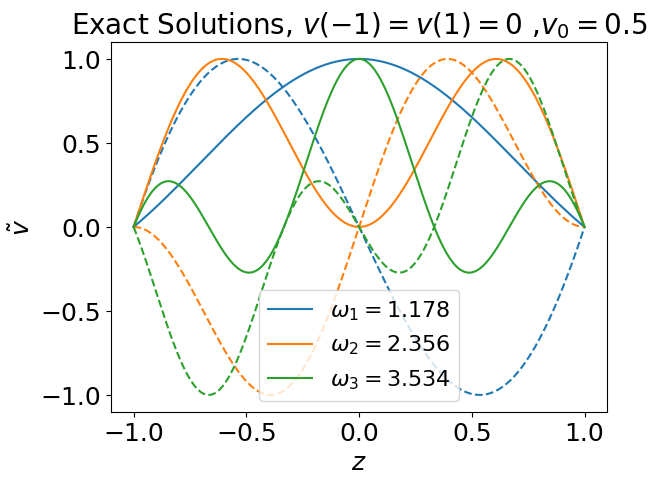
\includegraphics[width=\linewidth]{figures/exact-fixed-fixed-v0=0.5}
		\caption{Subsonic}
	\end{subfigure}%
	\begin{subfigure}{0.5\textwidth}
		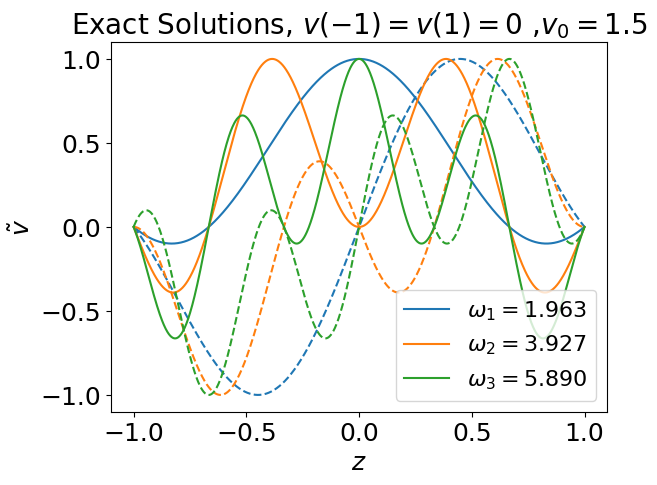
\includegraphics[width=\linewidth]{figures/exact-fixed-fixed-v0=1.5}
		\caption{Supersonic}
	\end{subfigure}
	\caption{The plots show the first three non-zero exact solutions to Eq.~(\ref{eq:constant-v-problem-dirichlet}) for both subsonic and supersonic case. These solutions are stable.}
	\label{fig:exact-v-dirichlet}
\end{figure}

\subsection{Fixed-Open Boundary}
Fixed-Open boundary condition assumes that there are no perturbations at the entrance of the nozzle, and it is free on the exit of the nozzle.

\begin{equation} \label{eq:constant-v-problem-fixed-open}
	\omega^2\tilde{v} + 2i\omega v_0\pdv{\tilde{v}}{z} + (1-v_0^2)\pdv[2]{\tilde{v}}{z} = 0
	\quad
	\tilde{v}(-1) = \pdv{\tilde{v}}{z}\,(1) = 0
\end{equation}

The solution to this problem is similar to Eq.~(\ref{eq:constant-v-solution-dirichlet}), the only difference is the eigenvalues. In this case, the eigenvalues are
\begin{equation}
	\omega_n = (v_0^2 - 1) \left[\frac{n\pi}{2} - \frac{1}{4}i\ln\abs{\frac{v_0-1}{v_0+1}}\right], \quad n\in\mathbb{Z}
	\label{eq:eigvals-constant-v-fixed-open}
\end{equation}
Again, the derivation can be found in Appendix.~\ref{chap:analytical-solutions}. The growth rate is independent of the mode number $n$, and it is always $\ln\abs{(v_0-1)/(v_0+1)}$. It is is positive for any $v_0\neq 1$. Therefore,
\begin{itemize}
	\item If $v_0<1$, then $\Im(\omega)<0$, it's damped oscillation, hence stable.
	\item If $v_0>1$, then $\Im(\omega)>0$, it's unstable.
\end{itemize}

\begin{figure}[htbp]
	\centering
	\begin{subfigure}{0.5\textwidth}
		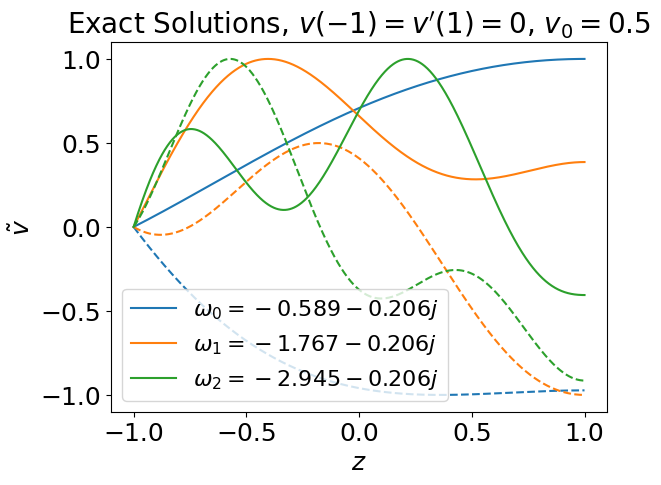
\includegraphics[width=\linewidth]{figures/exact-fixed-open-v0=0.5}
		\caption{Subsonic, stable flow.}
	\end{subfigure}%
	\begin{subfigure}{0.5\textwidth}
		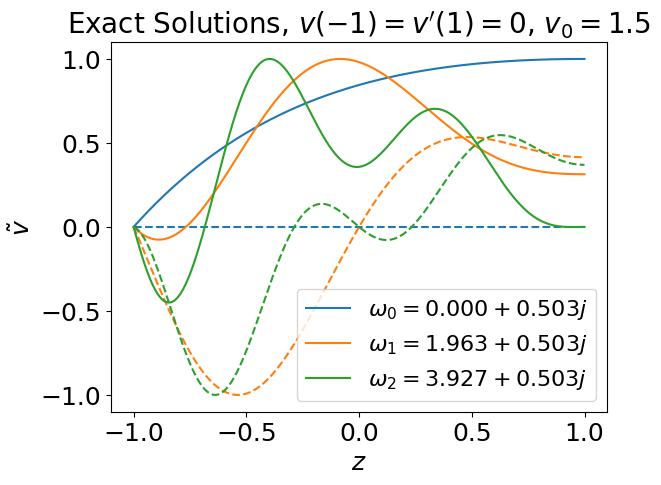
\includegraphics[width=\linewidth]{figures/exact-fixed-open-v0=1.5}
		\caption{Supersonic, unstable flow.}
	\end{subfigure}
	\caption{The plots show the first three exact solutions to Eq.~(\ref{eq:constant-v-problem-fixed-open}) for both subsonic and supersonic case. The flow is stable for subsonic case and unstable for supersonic case.}
	\label{fig:exact-v-fixed-open}
\end{figure}
